% ════════════════════════════════════════════════════════════════
\section{Wykład 14}
% ════════════════════════════════════════════════════════════════

Kontynuujemy temat najliczniejszego skojarzenia w grafach dwudzielnych. \\
$G = (V_1, V_2; E)$ -- graf dwudzielny. \\
\textbf{Instancja:} $G = (V_1, V_2; E)$. \\
\textbf{Problem:} Znaleźć najliczniejsze skojarzenie w $G$.

Niech $M$ będzie skojarzeniem w $G$. \\
Definiujemy graf skierowany $G_M = (V_1 \cup V_2, E_M)$, gdzie
\[
E_M = \{(u, v) : uv \in E - M,\ u \in V_1,\ v \in V_2\} \cup \{(v, u) : uv \in M,\ u \in V_1,\ v \in V_2\}.
\]
Innymi słowy, krawędzie wolne kierujemy z $V_1$ do $V_2$, a krawędzie skojarzone z $V_2$ do $V_1$.

\begin{example} ~ \\
	\begin{minipage}{0.48\textwidth}
		\centering
		\begin{tikzpicture}[x=0.9cm, y=0.9cm]
			\foreach \x/\name in {0/a, 1/b, 2/c, 3/d, 4/e} {
				\node[circle, fill=black, inner sep=1.5pt] (u\name) at (\x, 1) {};
			}
			\foreach \x/\name in {0/p, 1/q, 2/r, 3/s, 4/t} {
				\node[circle, fill=black, inner sep=1.5pt] (l\name) at (\x, 0) {};
			}
			\node[right] at (4.3, 1) {$V_1$};
			\node[right] at (4.3, 0) {$V_2$};
			\node[left] at (-0.3, 0.5) {$G$};
			
			
			\draw (ua) -- (lq);
			\draw (ub) -- (lp);
			\draw (uc) -- (lp);
			\draw[line width=1.5pt, accent] (uc) -- (lq);
			\draw (uc) -- (lr);
			\draw (uc) -- (ls);
			\draw (ud) -- (lr);
			\draw[line width=1.5pt, accent] (ud) -- (lt);
			\draw (ue) -- (ls);
			\draw (ue) -- (lt);
		\end{tikzpicture}
	\end{minipage}\hfill
	\begin{minipage}{0.48\textwidth}
		\centering
		\begin{tikzpicture}[x=0.9cm, y=0.9cm, >=stealth]
			\foreach \x/\name in {0/a, 1/b, 2/c, 3/d, 4/e} {
				\node[circle, fill=black, inner sep=1.5pt] (u\name) at (\x, 1) {};
			}
			\foreach \x/\name in {0/p, 1/q, 2/r, 3/s, 4/t} {
				\node[circle, fill=black, inner sep=1.5pt] (l\name) at (\x, 0) {};
			}
			\node[right] at (4.3, 1) {$V_1$};
			\node[right] at (4.3, 0) {$V_2$};
			\node[left] at (-0.3, 0.5) {$G_M$};
			
			% wolne wierzchołki w V_1: idc
			%\draw[draw=black] (ub) circle (4pt);
			%\draw[draw=black] (ue) circle (4pt);
			% wolne wierzchołki w V_2: idc
			%\draw[draw=black] (lp) circle (4pt);
			%\draw[draw=black] (lt) circle (4pt);
			
			\draw[->] (ua) -- (lq);
			\draw[->] (ub) -- (lp);
			\draw[->] (uc) -- (lp);
			\draw[<-, line width=1.2pt, accent] (uc) -- (lq);
			\draw[->] (uc) -- (lr);
			\draw[->] (uc) -- (ls);
			\draw[->] (ud) -- (lr);
			\draw[<-, line width=1.2pt, accent] (ud) -- (lt);
			\draw[->] (ue) -- (ls);
			\draw[->] (ue) -- (lt);
			
			% krawędzie wolne: V_1 -> V_2
			% krawędzie skojarzone: V_2 -> V_1
		\end{tikzpicture}
	\end{minipage}
	
	%\vspace{0.5em}
	%\noindent Symbol $\bigodot$ oznacza wolny wierzchołek.
\end{example}

Oto procedura do znajdowania ścieżki powiększającej -- Augmenting Path Search (APS).

\begin{alg}{Augmenting Path Search}{alg:aps:lect14}
	\FunctionNN{APS}{$G, M$} \Comment{$G = (V_1, V_2; E)$, $M$ -- skojarzenie w $G$}
	\State $V_1'$ \Assign zbiór wierzchołków wolnych z $V_1$
	\State $V_2'$ \Assign zbiór wierzchołków wolnych z $V_2$
	\State skonstruuj graf skierowany $G_M = (V_1 \cup V_2, E_M)$
	\State znajdź ścieżkę $\vec{P}$ z $V_1'$ do $V_2'$ w $G_M$
	\If{$\vec{P}$ istnieje}
	\State \Return $P$ \Comment{$P$ -- nieskierowana $\vec{P}$}
	\Else
	\State \Return NULL
	\EndIf
	\EndFunction
\end{alg}

\begin{lemma}
	Procedura \textnormal{APS} zwraca ścieżkę $P \iff$ istnieje ścieżka powiększająca względem $M$ w $G$. Ponadto ścieżka $P$ zwrócona przez \textnormal{APS} jest ścieżką powiększającą względem $M$.
\end{lemma}

\begin{proof}~\\
	$\implies$ Jeśli \textnormal{APS} zwraca ścieżkę $P$, to skierowana ścieżka $\vec{P}$ znaleziona w linii 4 zaczyna się w wierzchołku z $V_1'$ (a więc wolnym) i kończy się w wierzchołku z $V_2'$ (a więc wolnym). Z definicji grafu $G_M$ wynika, że pierwsza krawędź $P$ jest wolna, druga krawędź $P$ jest skojarzona, trzecia krawędź $P$ jest wolna, \dots, ostatnia krawędź $P$ jest wolna. Zatem $P$ jest ścieżką powiększającą względem $M$.
	
	$\impliedby$ Jeśli istnieje ścieżka powiększająca względem $M$ w $G$, to ścieżka skierowana otrzymana z takiej ścieżki powiększającej przez skierowanie krawędzi zgodnie z $E_M$ jest ścieżką skierowaną z $V_1'$ do $V_2'$ w $G_M$. Taką ścieżkę skierowaną znajduje \textnormal{APS}.
\end{proof}

Oto algorytm znajdowania najliczniejszego skojarzenia -- Maximum Matching (MM).

\begin{alg}{Maximum Matching}{alg:mm:lect14}
	\FunctionNN{MM}{$G$} \Comment{$G = (V_1, V_2; E)$}
	\State $M \Assign \emptyset$
	\Repeat
	\State $P \Assign \Call{APS}{G, M}$
	\If{$P \neq$ NULL}
	\State $M \Assign M \div E(P)$
	\EndIf
	\Until{$P =$ NULL}
	\State \Return $M$
	\EndFunction
\end{alg}

\paragraph{Poprawność.} Wynika z twierdzenia Berge'a.

\paragraph{Złożoność czasowa.}

Złożoność czasowa \textnormal{APS}:
\begin{flalign*}
	& \text{linie } 1, 2 \quad && \BO(|V|) && \\
	& \text{linia } 3 \quad && \BO(|E|) && \\
	& \text{linia } 4 \quad && \BO(|E|) \text{ -- BFS} && \\
	& \text{linie } 5\text{--}8 \quad && \BO(|V|) &&
\end{flalign*}
Złożoność \textnormal{APS} wynosi $\BO(|E|)$.

Złożoność czasowa \textnormal{MM}:
\begin{itemize}[nosep]
	\item Linia 1: $\BO(1)$.
	\item Pętla 2--6 wykona się co najwyżej $\frac{|V|}{2}$ razy, bo w każdej iteracji $|M|$ zwiększa się o $1$, a maksymalna liczność skojarzenia jest $\le \frac{|V|}{2}$.
	\item Wnętrze pętli:
	\begin{flalign*}
		& \text{linia } 3 \quad && \BO(|E|) && \\
		& \text{linia } 5 \quad && \BO(|V|) &&
	\end{flalign*}
	Razem $\BO(|E|)$.
	\item Linia 7: $\BO(|V|)$.
\end{itemize}
Ostateczna złożoność \textnormal{MM} wynosi $\BO(|V| \cdot |E|)$.

\paragraph{Przykład.} Prześledźmy działanie algorytmu \textnormal{MM} na poniższym grafie $G$:

\definecolor{path}{RGB}{250, 0, 135}
\begin{figure}[H]
	\centering
	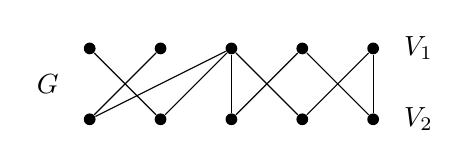
\begin{tikzpicture}[x=0.9cm, y=0.9cm]
		\foreach \x/\name in {0/a, 1/b, 2/c, 3/d, 4/e} {
			\node[circle, fill=black, inner sep=1.5pt] (u\name) at (\x, 1) {};
		}
		\foreach \x/\name in {0/p, 1/q, 2/r, 3/s, 4/t} {
			\node[circle, fill=black, inner sep=1.5pt] (l\name) at (\x, 0) {};
		}
		\node[right] at (4.3, 1) {$V_1$};
		\node[right] at (4.3, 0) {$V_2$};
		\node[left] at (-0.3, 0.5) {$G$};
		
		\draw (ua) -- (lq);
		\draw (ub) -- (lp);
		\draw (uc) -- (lp);
		\draw (uc) -- (lq);
		\draw (uc) -- (lr);
		\draw (uc) -- (ls);
		\draw (ud) -- (lr);
		\draw (ud) -- (lt);
		\draw (ue) -- (ls);
		\draw (ue) -- (lt);
	\end{tikzpicture}
\end{figure}

\noindent\textbf{Iteracja 1:}
\begin{figure}[H]
	\centering
	\begin{minipage}{0.48\linewidth}
		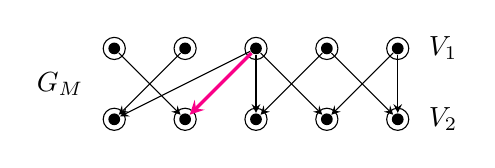
\begin{tikzpicture}[x=0.9cm, y=0.9cm, >=stealth]
			\foreach \x/\name in {0/a, 1/b, 2/c, 3/d, 4/e} {
				\node[circle, fill=black, inner sep=1.5pt] (u\name) at (\x, 1) {};
			}
			\foreach \x/\name in {0/p, 1/q, 2/r, 3/s, 4/t} {
				\node[circle, fill=black, inner sep=1.5pt] (l\name) at (\x, 0) {};
			}
			\node[right] at (4.3, 1) {$V_1$};
			\node[right] at (4.3, 0) {$V_2$};
			\node[left] at (-0.3, 0.5) {$G_M$};
			
			% wszystkie wolne
			\foreach \name in {a, b, c, d, e} {\draw[draw=black] (u\name) circle (4pt);}
			\foreach \name in {p, q, r, s, t} {\draw[draw=black] (l\name) circle (4pt);}
			
			
			\draw[->] (ua) -- (lq);
			\draw[->] (ub) -- (lp);
			\draw[->] (uc) -- (lp);
			\draw[->, line width=1.2pt, path] (uc) -- (lq);
			\draw[->] (uc) -- (lr);
			\draw[->] (uc) -- (ls);
			\draw[->] (ud) -- (lr);
			\draw[->] (ud) -- (lt);
			\draw[->] (ue) -- (ls);
			\draw[->] (ue) -- (lt);
		\end{tikzpicture}
	\end{minipage}\hfill\begin{minipage}{0.48\linewidth}
		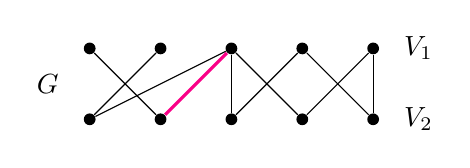
\begin{tikzpicture}[x=0.9cm, y=0.9cm, >=stealth]
			\foreach \x/\name in {0/a, 1/b, 2/c, 3/d, 4/e} {
				\node[circle, fill=black, inner sep=1.5pt] (u\name) at (\x, 1) {};
			}
			\foreach \x/\name in {0/p, 1/q, 2/r, 3/s, 4/t} {
				\node[circle, fill=black, inner sep=1.5pt] (l\name) at (\x, 0) {};
			}
			\node[right] at (4.3, 1) {$V_1$};
			\node[right] at (4.3, 0) {$V_2$};
			\node[left] at (-0.3, 0.5) {$G$};
			
			\draw (ua) -- (lq);
			\draw (ub) -- (lp);
			\draw (uc) -- (lp);
			\draw[line width=1.2pt, path] (uc) -- (lq);
			\draw (uc) -- (lr);
			\draw (uc) -- (ls);
			\draw (ud) -- (lr);
			\draw (ud) -- (lt);
			\draw (ue) -- (ls);
			\draw (ue) -- (lt);
		\end{tikzpicture}
	\end{minipage} 
\end{figure}

\noindent\textbf{Iteracja 2:}

\begin{figure}[H]
	\centering
	\begin{minipage}{0.48\linewidth}
		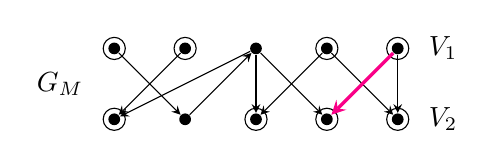
\begin{tikzpicture}[x=0.9cm, y=0.9cm, >=stealth]
			\foreach \x/\name in {0/a, 1/b, 2/c, 3/d, 4/e} {
				\node[circle, fill=black, inner sep=1.5pt] (u\name) at (\x, 1) {};
			}
			\foreach \x/\name in {0/p, 1/q, 2/r, 3/s, 4/t} {
				\node[circle, fill=black, inner sep=1.5pt] (l\name) at (\x, 0) {};
			}
			\node[right] at (4.3, 1) {$V_1$};
			\node[right] at (4.3, 0) {$V_2$};
			\node[left] at (-0.3, 0.5) {$G_M$};
			
			\foreach \name in {a, b, d, e} {\draw[draw=black] (u\name) circle (4pt);}
			\foreach \name in {p, r, s, t} {\draw[draw=black] (l\name) circle (4pt);}
			
			
			\draw[->] (ua) -- (lq);
			\draw[->] (ub) -- (lp);
			\draw[->] (uc) -- (lp);
			\draw[<-] (uc) -- (lq);
			\draw[->] (uc) -- (lr);
			\draw[->] (uc) -- (ls);
			\draw[->] (ud) -- (lr);
			\draw[->] (ud) -- (lt);
			\draw[->, line width=1.2pt, path] (ue) -- (ls);
			\draw[->] (ue) -- (lt);
		\end{tikzpicture}
	\end{minipage}\hfill\begin{minipage}{0.48\linewidth}
		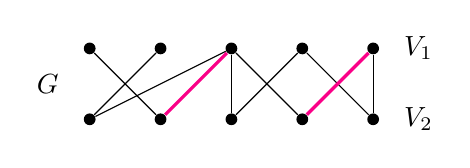
\begin{tikzpicture}[x=0.9cm, y=0.9cm, >=stealth]
			\foreach \x/\name in {0/a, 1/b, 2/c, 3/d, 4/e} {
				\node[circle, fill=black, inner sep=1.5pt] (u\name) at (\x, 1) {};
			}
			\foreach \x/\name in {0/p, 1/q, 2/r, 3/s, 4/t} {
				\node[circle, fill=black, inner sep=1.5pt] (l\name) at (\x, 0) {};
			}
			\node[right] at (4.3, 1) {$V_1$};
			\node[right] at (4.3, 0) {$V_2$};
			\node[left] at (-0.3, 0.5) {$G$};
			
			\draw (ua) -- (lq);
			\draw (ub) -- (lp);
			\draw (uc) -- (lp);
			\draw[line width=1.2pt, path] (uc) -- (lq);
			\draw (uc) -- (lr);
			\draw (uc) -- (ls);
			\draw (ud) -- (lr);
			\draw (ud) -- (lt);
			\draw[line width=1.2pt, path] (ue) -- (ls);
			\draw (ue) -- (lt);
		\end{tikzpicture}
	\end{minipage} 
\end{figure}

\noindent\textbf{Iteracja 3:}

\begin{figure}[H]
	\centering
	\begin{minipage}{0.48\linewidth}
		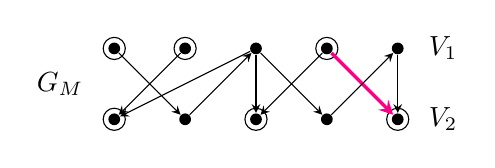
\begin{tikzpicture}[x=0.9cm, y=0.9cm, >=stealth]
			\foreach \x/\name in {0/a, 1/b, 2/c, 3/d, 4/e} {
				\node[circle, fill=black, inner sep=1.5pt] (u\name) at (\x, 1) {};
			}
			\foreach \x/\name in {0/p, 1/q, 2/r, 3/s, 4/t} {
				\node[circle, fill=black, inner sep=1.5pt] (l\name) at (\x, 0) {};
			}
			\node[right] at (4.3, 1) {$V_1$};
			\node[right] at (4.3, 0) {$V_2$};
			\node[left] at (-0.3, 0.5) {$G_M$};
			
			\foreach \name in {a, b, d} {\draw[draw=black] (u\name) circle (4pt);}
			\foreach \name in {p, r, t} {\draw[draw=black] (l\name) circle (4pt);}
			
			
			\draw[->] (ua) -- (lq);
			\draw[->] (ub) -- (lp);
			\draw[->] (uc) -- (lp);
			\draw[<-] (uc) -- (lq);
			\draw[->] (uc) -- (lr);
			\draw[->] (uc) -- (ls);
			\draw[->] (ud) -- (lr);
			\draw[->, line width=1.2pt, path] (ud) -- (lt);
			\draw[<-] (ue) -- (ls);
			\draw[->] (ue) -- (lt);
		\end{tikzpicture}
	\end{minipage}\hfill\begin{minipage}{0.48\linewidth}
		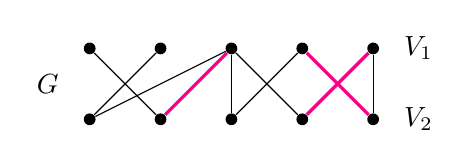
\begin{tikzpicture}[x=0.9cm, y=0.9cm, >=stealth]
			\foreach \x/\name in {0/a, 1/b, 2/c, 3/d, 4/e} {
				\node[circle, fill=black, inner sep=1.5pt] (u\name) at (\x, 1) {};
			}
			\foreach \x/\name in {0/p, 1/q, 2/r, 3/s, 4/t} {
				\node[circle, fill=black, inner sep=1.5pt] (l\name) at (\x, 0) {};
			}
			\node[right] at (4.3, 1) {$V_1$};
			\node[right] at (4.3, 0) {$V_2$};
			\node[left] at (-0.3, 0.5) {$G$};
			
			\draw (ua) -- (lq);
			\draw (ub) -- (lp);
			\draw (uc) -- (lp);
			\draw[line width=1.2pt, path] (uc) -- (lq);
			\draw (uc) -- (lr);
			\draw (uc) -- (ls);
			\draw (ud) -- (lr);
			\draw[line width=1.2pt, path] (ud) -- (lt);
			\draw[line width=1.2pt, path] (ue) -- (ls);
			\draw (ue) -- (lt);
		\end{tikzpicture}
	\end{minipage} 
\end{figure}


\noindent\textbf{Iteracja 4:}

\begin{figure}[H]
	\centering
	\begin{minipage}{0.48\linewidth}
		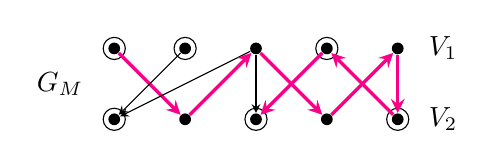
\begin{tikzpicture}[x=0.9cm, y=0.9cm, >=stealth]
			\foreach \x/\name in {0/a, 1/b, 2/c, 3/d, 4/e} {
				\node[circle, fill=black, inner sep=1.5pt] (u\name) at (\x, 1) {};
			}
			\foreach \x/\name in {0/p, 1/q, 2/r, 3/s, 4/t} {
				\node[circle, fill=black, inner sep=1.5pt] (l\name) at (\x, 0) {};
			}
			\node[right] at (4.3, 1) {$V_1$};
			\node[right] at (4.3, 0) {$V_2$};
			\node[left] at (-0.3, 0.5) {$G_M$};
			
			\foreach \name in {a, b, d} {\draw[draw=black] (u\name) circle (4pt);}
			\foreach \name in {p, r, t} {\draw[draw=black] (l\name) circle (4pt);}
			
			
			\draw[->, line width=1.2pt, path] (ua) -- (lq);
			\draw[->] (ub) -- (lp);
			\draw[->] (uc) -- (lp);
			\draw[<-, line width=1.2pt, path] (uc) -- (lq);
			\draw[->] (uc) -- (lr);
			\draw[->, line width=1.2pt, path] (uc) -- (ls);
			\draw[->, line width=1.2pt, path] (ud) -- (lr);
			\draw[<-, line width=1.2pt, path] (ud) -- (lt);
			\draw[<-, line width=1.2pt, path] (ue) -- (ls);
			\draw[->, line width=1.2pt, path] (ue) -- (lt);
		\end{tikzpicture}
	\end{minipage}\hfill\begin{minipage}{0.48\linewidth}
		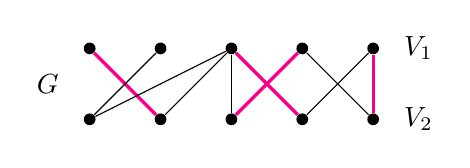
\begin{tikzpicture}[x=0.9cm, y=0.9cm, >=stealth]
			\foreach \x/\name in {0/a, 1/b, 2/c, 3/d, 4/e} {
				\node[circle, fill=black, inner sep=1.5pt] (u\name) at (\x, 1) {};
			}
			\foreach \x/\name in {0/p, 1/q, 2/r, 3/s, 4/t} {
				\node[circle, fill=black, inner sep=1.5pt] (l\name) at (\x, 0) {};
			}
			\node[right] at (4.3, 1) {$V_1$};
			\node[right] at (4.3, 0) {$V_2$};
			\node[left] at (-0.3, 0.5) {$G$};
			
			\draw[line width=1.2pt, path] (ua) -- (lq);
			\draw (ub) -- (lp);
			\draw (uc) -- (lp);
			\draw[] (uc) -- (lq);
			\draw (uc) -- (lr);
			\draw[line width=1.2pt, path] (uc) -- (ls);
			\draw[line width=1.2pt, path] (ud) -- (lr);
			\draw[] (ud) -- (lt);
			\draw[] (ue) -- (ls);
			\draw[line width=1.2pt, path] (ue) -- (lt);
		\end{tikzpicture}
	\end{minipage} 
\end{figure}

\noindent\textbf{Iteracja 5:}


\begin{figure}[H]
	\centering
	\begin{minipage}{0.48\linewidth}
		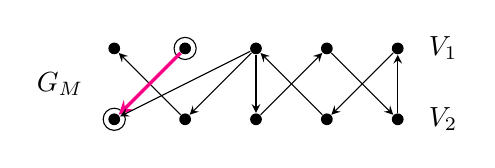
\begin{tikzpicture}[x=0.9cm, y=0.9cm, >=stealth]
			\foreach \x/\name in {0/a, 1/b, 2/c, 3/d, 4/e} {
				\node[circle, fill=black, inner sep=1.5pt] (u\name) at (\x, 1) {};
			}
			\foreach \x/\name in {0/p, 1/q, 2/r, 3/s, 4/t} {
				\node[circle, fill=black, inner sep=1.5pt] (l\name) at (\x, 0) {};
			}
			\node[right] at (4.3, 1) {$V_1$};
			\node[right] at (4.3, 0) {$V_2$};
			\node[left] at (-0.3, 0.5) {$G_M$};
			
			\foreach \name in {b} {\draw[draw=black] (u\name) circle (4pt);}
			\foreach \name in {p} {\draw[draw=black] (l\name) circle (4pt);}
			
			
			\draw[<-] (ua) -- (lq);
			\draw[->, line width=1.2pt, path] (ub) -- (lp);
			\draw[->] (uc) -- (lp);
			\draw[->] (uc) -- (lq);
			\draw[->] (uc) -- (lr);
			\draw[<-] (uc) -- (ls);
			\draw[<-] (ud) -- (lr);
			\draw[->] (ud) -- (lt);
			\draw[->] (ue) -- (ls);
			\draw[<-] (ue) -- (lt);
		\end{tikzpicture}
	\end{minipage}\hfill\begin{minipage}{0.48\linewidth}
		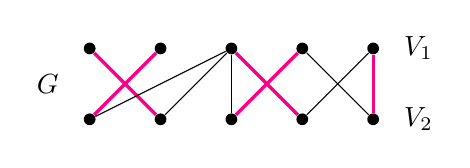
\begin{tikzpicture}[x=0.9cm, y=0.9cm, >=stealth]
			\foreach \x/\name in {0/a, 1/b, 2/c, 3/d, 4/e} {
				\node[circle, fill=black, inner sep=1.5pt] (u\name) at (\x, 1) {};
			}
			\foreach \x/\name in {0/p, 1/q, 2/r, 3/s, 4/t} {
				\node[circle, fill=black, inner sep=1.5pt] (l\name) at (\x, 0) {};
			}
			\node[right] at (4.3, 1) {$V_1$};
			\node[right] at (4.3, 0) {$V_2$};
			\node[left] at (-0.3, 0.5) {$G$};
			
			\draw[line width=1.2pt, path] (ua) -- (lq);
			\draw[line width=1.2pt, path] (ub) -- (lp);
			\draw (uc) -- (lp);
			\draw[] (uc) -- (lq);
			\draw (uc) -- (lr);
			\draw[line width=1.2pt, path] (uc) -- (ls);
			\draw[line width=1.2pt, path] (ud) -- (lr);
			\draw[] (ud) -- (lt);
			\draw[] (ue) -- (ls);
			\draw[line width=1.2pt, path] (ue) -- (lt);
		\end{tikzpicture}
	\end{minipage} 
\end{figure}